
%                                  127
\noindent\textbf{7. Правильный пятиугольник для всех (без Ферма и Гаусса)}\\

Зная, что
\begin{center}
$-cos\dfrac{\pi}{5}=cos\dfrac{4\pi}{5}=2cos^2\dfrac{2\pi}{5}-1=8cos^4\dfrac{\pi}{5}-8cos^2\dfrac{\pi}{5}+1$,
\end{center}
достаточно разложить на множители многочлен $8X^4-8X^2+X+1$\linebreak
(очевидными корнями которого являются —1 и 1/2). Единственное до-\linebreak
пустимое решение для $cos\dfrac{\pi}{5}$ - это $\dfrac{1+\sqrt{5}}{4}$. Тогда построение проводится\linebreak
следующим способом (см. рис. 2):\\

\begin{wrapfigure}{i}{0.5\textwidth}
\begin{center}
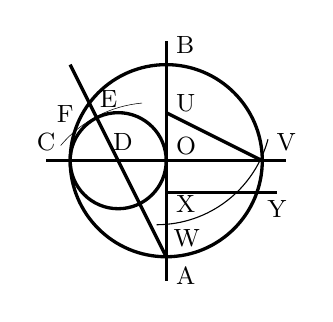
\begin{tikzpicture} [scale = 0.61]
\coordinate [label=right:\small{A}] (A) at (0, -2.4);
\coordinate [label=right:\small{B}] (B) at (0, 2.4);
\coordinate [label=above:\small{C}] (C) at (-2.5, 0);
\coordinate [label=above:\small{D}] (D) at (-0.9, 0);
\coordinate [label=above:\small{E}] (E) at (-1.2, 0.9);
\coordinate [label=above:\small{F}] (F) at (-2.1, 0.6);
\coordinate [label=right:\small{O}] (O) at (0, 0.3);
\coordinate [label=right:\small{U}] (U) at (0, 1.2);
\coordinate [label=above:\small{V}] (V) at (2.5, 0);
\coordinate [label=right:\small{W}] (W) at (-0.05, -1.6);
\coordinate [label=right:\small{X}] (X) at (0, -0.9);
\coordinate [label=right:\small{Y}] (Y) at (1.9, -1);
\draw[very thick] (0, 0) circle (2); %big circle
\draw[very thick] (-1, 0) circle (1); %small circle
\draw[thin] (-0.2, -4/3) arc (270:345:2.4); %WV
\draw[very thin] (-0.5, 1.2) arc (95:140:2.5); %FE
\draw[very thick] (-2.5, 0) -- (2.5, 0); %CV line
\draw[very thick] (0, -2.5) -- (0, 2.5); %AB line
\draw[very thick] (0, 1) -- (2, 0); %UV line
\draw[very thick] (0, -2/3) -- (2.3, -2/3); %XY line
\draw[very thick] (0, -2) -- (-2, 2); %AE line
\end{tikzpicture}\\
\textbf{Рис.2} Правильный пятиугольник
\end{center}
\end{wrapfigure}
\noindent
$\bullet$ построить окружность с це-\linebreak
тром $O$ и радиусом 1,\newline
$\bullet$ построить диаметр $AB$, ра-\linebreak
диус $OC$ перпендикулярно $AB$\linebreak
и окружность радиусом $1/2$ с\linebreak
центром в $D$ - середине $OC$,\newline
$\bullet$ прямая $AD$ делит эту окруж-\linebreak
ность в двух точках, из кото-\linebreak
рых наиболее удаленная от $A$\linebreak
точка $E$ удовлетворяет усло-\linebreak
вию: $AE=\phi(AD=\sqrt{5}/2)$ и\linebreak
$DE=1/2)$.\newline
Тогда достаточно постро-\linebreak
ить на окружности радиуса 1
с центром $O$ точку $F$ такую, что $AF=\phi$, и получаем прямоугольный
треугольник, в котором угол $(\widehat{FAB})$ равен $\pi/5$.\newline
\hspace*{15pt}Соответствующий центральный угол$(\widehat{FOB})$ равен $2\pi/5$ и позволяет\linebreak
построить правильный пятиугольник (Слейе-Мишо[48]).\newline
Существуют и другие решения, и вот одно из них, особенно про-\linebreak
стое: если $z$ есть корень 5-й степени из единицы, соотношение $z^4+$\linebreak
$z^3+z^2+z+1=0$ приводит к тригонометрическому уравнению\linebreak
$2cos\dfrac{2\pi}{5}+2cos\dfrac{4\pi}{5}+1=0$, которое просто решается, давая $cos\dfrac{2\pi}{5}=\dfrac{\sqrt{5}-1}{4}$.\linebreak
Сразу осуществимо построение. Если $U$ — середина $OB$, строим точ-\linebreak
ку $W$ , расположенную на радиусе $OA$ и удовлетворяющую равенству\linebreak
$UW=UV=\sqrt{5}/2$. Точка $X$ , середина $OW$, есть ортогональная проек-\linebreak
ция точки $Y$ такой, что угол $(\widehat{AOY})$ равен $2\pi/5$.
\noindent\textbf{8. <<Двоичное>> деление нацело}
\hspace*{15pt}\textbf{a.} Вот евклидово деление $a$ на $2b$: $a=2b\times q+r$, с $0\leqslant r<2b$. Если\linebreak
$r<b$, то евклидово деление $a$ на $b$ получается сразу: $a=b\times 2q+r$. Зато,\linebreak
если $b\leqslant r<2b$, деление таково: $a=b\times(2q+1)+(r-b)$.
\newpage


%                                  128
\textbf{b.} Предельный случай евклидова деления появляется, когда дели-\linebreak
тель больше делимого. Вот рекурсивный алгоритм вычисления частно-\linebreak
го и остатка, представленный в форме функции $Divide$:
\begin{lstlisting}[frame=single, mathescape=true]
if ($b$ > $a$)  return $(0,a)$;
else {
  $(q,r) \longleftarrow$ Divide $(a,2b)$;
  if ($r$ < $b$)  return $(2q,r)$;
  else  return $(2q+1,r-b)$; }
\end{lstlisting}
\hspace*{15pt}\textbf{d.} Недостаток рекурсивного алгоритма следующий: в ходе счета\linebreak
второй параметр функции $Divide$, который удваивается при каждом\linebreak
вызове, может превзойти первоначальные величины переменных $a$ и $b$.\linebreak
Это означает, что хотя данные и результат деления поддаются коди-\linebreak
рованию, может случиться, что в какой-либо частной реализации вели-\linebreak
чины приведут к переполнению.\newline
\hspace*{15pt}Например, когда применяют рекурсивный алгоритм к целым чи-\linebreak
слам 31001 и 15, наблюдается ряд рекурсивных вызовов, последний из\linebreak
которых — \textit{Divide}(31001,61440); если целый тип, который используют,\linebreak
записан и закодирован 16 битами, возникает переполнение, тогда как\linebreak
можно очень хорошо вычислить результат (2066,11), если остановить\linebreak
удвоение $b$ перед последней итерацией.\newline
\begin{center}
\begin{tabular}{|l|l|}
\hline
\hspace*{28pt}\underline{\textbf{A.} С переполнением}
&
\hspace*{23pt}\underline{\textbf{B.} Без переполнения}\\
{\begin{lstlisting}[mathescape=true, frame=none]
$k\longleftarrow0$;
if $b$ > $a$  return (0,$a$);
while ($b\leqslant a/2$) {
  $b\longleftarrow 2\times b$; $k\longleftarrow k+1$;
}
$q\longleftarrow 0$; $r\longleftarrow a$;
for (int $i$=1; $i\leqslant k+1$; ++$i$) {
  $q\longleftarrow 2\times q$;
  if ($r\geqslant b$) {
    $q\longleftarrow q+1$; $r\longleftarrow r-b$;
  }
  $b\longleftarrow b/2$;
}
return (q,r);
\end{lstlisting}}
&
{\begin{lstlisting}[mathescape=true, frame=none]
$k\longleftarrow 0$;
while ($b\leqslant a$) {
  $b\longleftarrow 2\times b$; $k\longleftarrow k+1$;
}
$q\longleftarrow 0$; $r\longleftarrow a$;
for (int $i=1$; $i\leqslant k$; ++$i$) {
  $b\longleftarrow b/2$; $q\longleftarrow 2\times q$;
  if ($r\geqslant b$) {
    $q\longleftarrow q+1$; $r\longleftarrow r-b$;
  }
}
\end{lstlisting}}\\
\hline
\end{tabular}
\end{center}
\begin{center}
\textbf{Алгоритм 8.} Бинарные деления
\end{center}
\newpage

%                                  129                            
Теперь уже можно — это пригодится в дальнейшем — написать\linebreak
итерационный алгоритм (8-А), который есть не что иное, как разви-\linebreak
тие предыдущего рекурсивного алгоритма ($q$ и $r$ образуют результат\linebreak
алгоритма: частное и остаток от деления). Этот алгоритм яснее вы-\linebreak
являет поставленную задачу.\\\\
\hspace*{15pt}\textbf{e.} Чтобы показать эквивалентность двух алгоритмов, можно на-\linebreak
чать с доказательства очень простого свойства: $[a/2]<b\Leftrightarrow a<2b$.\newline
\hspace*{15pt}На выходе из цикла первого алгоритма имеем свойство\linebreak
$b/2\leqslant a<b=b_02^k$ с $k>0$ - не забудем, что тело цикла использу-\linebreak
ется, по крайней мере, один раз.\newline
\hspace*{15pt}Что касается второго алгоритма, если цикл использовался, по край-\linebreak
ней мере, один раз, имеем свойство $b/2\leqslant a/2<b=b_02^k$ для $k>1$ и\linebreak
$b$ - четного. После выполнения последних присваиваний обнаруживаем\linebreak
то же свойство, что и для первого алгоритма. Если цикл не выполнен,\linebreak
это означает, что $a/2<b_0\leqslant a$, и после исполнения последних команд\linebreak
получаем $b_0=b/2\leqslant a<b=2b_0$.\newline
\hspace*{15pt}Последний алгоритм (8-В) получен, исходя из первой итерационной\linebreak
версии (8-А) извлечением из первого цикла итерации и ее слиянием с\linebreak
итерацией, взятой из второго цикла (для этого алгоритма, как и для\linebreak
предыдущего, результат - частное и остаток - представлен послед-\linebreak
ними значениями переменных $q$ и $r$).\\

\noindent\textbf{9. Построение прямых линий методами DDA}\\

\hspace*{15pt}\textbf{a.} Если $u$ и $v$ не взаимно простые числа, отрезок $[0, (u,v)]$ - не что\linebreak
иное, как повторение $d=$НОД$(u,v)$ сегментов, идентичных сегменту\linebreak
$[0,(u/d,v/d)]$.
\begin{center}
\begin{tabular}{|l|l|}
\hline
\hspace*{50pt}Алгоритм&
\hspace{5pt}Построение\\
{\begin{lstlisting}[mathescape=true, frame=none]
$y\longleftarrow 0$; $d\longleftarrow 0$; $Plot(0,0)$;
for (int $x=1$; $x\leqslant u$; ++$x$) {
  $2(vx-uy)=dc-u\leqslant d<u$.
  $d\longleftarrow d+2v$;
  if ($d\geqslant u$) {
    $y\longleftarrow y+1$; $d\longleftarrow d-2u$;
  }
  $Plot(x,y)$;
}
\end{lstlisting}}
&
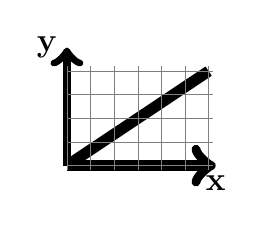
\begin{tikzpicture} [scale=0.3]
\coordinate [label=below:\textbf{\large{x}}] (x) at (6.3, 0);
\coordinate [label=left:\textbf{\large{y}}] (y) at (0, 5);
\draw[->, line width=3pt] (0, 0) to (y);
\draw[->, line width=4pt] (0, 0) to (x);
\draw[line width=4pt] (0, 0) -- (6, 4);
\draw[help lines] (0,-0.2) grid (6.2,4.2);<br>
\end{tikzpicture}\\
\hline
\end{tabular}
\end{center}
\begin{center}
\textbf{Рис. 3.} Построение прямой в первом октанте
\end{center}
\newpage


%                                  130
\textbf{b.} Выбрать для $y$ наилучшую целую аппроксимацию величины $vx/u$\linebreak
- это значит убедиться, что $|vx/u-y|\leqslant 1/2$, или еще, что\linebreak
$-u\leqslant2(vx-uy)<u$. Эта формула является в действительности ин-\linebreak
вариантом алгоритма. Поскольку нужная прямая имеет тангенс угла\linebreak
наклона меньше 1, есть только один зажигающийся пиксел на данной\linebreak
вертикали (т.е. $х$ возрастает при каждой итерации). Этот алгоритм\linebreak
(рис. 3) избегает, следовательно, пересечений маленьких горизонталь-\linebreak
ных сегментов, что дает красивый результат, когда нужны тонкие ли-\linebreak
нии; было бы совсем по-другому, если нужно <<жирное>> построение.\newline
\hspace*{15pt}Кроме того, если желаем построить этим способом прямую с накло-\linebreak
ном, большим 1, нужен второй алгоритм, идентичный первому с точ-\linebreak
ностью до перемены ролями $x$ и $y$. Наконец, построение вертикальных,\linebreak
горизонтальных или диагональных линий может проводиться наивным\linebreak
способом, который будет всегда более быстрым, чем указанный.\newline
\begin{center}
\begin{tabular}{|l|l|}
\hline
\hspace*{50pt}Алгоритм&
\hspace{5pt}Построение\\
{\begin{lstlisting}[mathescape=true, frame=none]
$x\longleftarrow 0$; $y\longleftarrow 0$; $d\longleftarrow v-u$;
for (;;) {
  $Plot(x,y)$
  $d=\delta(x,y+v-u c |\delta(x,y)|\leqslant u+v)$.
  if ($d>0$) {
    $y\longleftarrow y+1$; $d\longleftarrow d-2u$;
  } else {
    $x\longleftarrow x+1$; $d\longleftarrow d+2v$;
  }
  if (($x$==$u$) && ($y$==$v$))  break;
}
$Plot(x,y)$;
\end{lstlisting}}
&
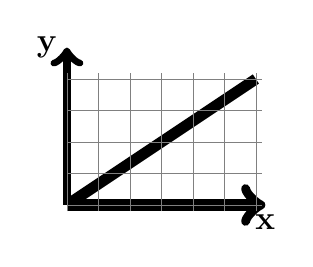
\begin{tikzpicture}[scale=0.4]
\coordinate [label=below:\textbf{\large{x}}] (x) at (6.3, 0);
\coordinate [label=left:\textbf{\large{y}}] (y) at (0, 5);
\draw[->, line width=3pt] (0, 0) to (y);
\draw[->, line width=4pt] (0, 0) to (x);
\draw[line width=4pt] (0, 0) -- (6, 4);
\draw[help lines] (0,-0.2) grid (6.2,4.2);<br>
\end{tikzpicture}\\
\hline
\end{tabular}
\end{center}
\begin{center}
\textbf{Рис. 4.} Построение прямой в первой четверти
\end{center}
\hspace*{15pt}\textbf{c.} Парадоксально, но этот алгоритм (рис. 4) - который может\linebreak
дать менее элегантные результаты, чем предыдущий, - оказывается\linebreak
немного более сложным для реализации. Действительно, нельзя больше\linebreak
предполагать, что координата $x$ возрастает после включения точки; на\linebreak
самом деле, каждая координата является \textit{доминантой} в полуквадран-\linebreak
те, о котором рассуждаем. Если рассмотреть четыре точки квадрата,\linebreak
сразу замечаем, что невозможно требовать - если не разрешены диаго-\linebreak
нальные перемещения - чтобы вертикальное расстояние правой точки\linebreak
было меньше $1/2$. Если поддерживать включенную точку в полосе фи-\linebreak
гуры 1, это влечет, между прочим, что одно из расстояний справа, го-\linebreak
\newpage


%                                  131
\noindent
ризонтальное или вертикальное, может быть сохранено меньшим 1, это\linebreak
означает, что величина $|vx-uy|$ меньше, чем $u$ или $v$. Сказать, что точ-\linebreak
ка расположена в полосе, очень точно означает, что $|2(vx-uy)|\leqslant u+v$;\linebreak
теперь покажем, что можно подтвердить это положение.\newline
\hspace*{15pt}Движение, осуществляемое на экране, будет определяться величи-\linebreak
ной $\delta(x,y)=2(vx-uy)$, получаемой после этого движения. Возможны\linebreak
два (не исключительных) случая: увеличивают $x$, величина становится\linebreak
равной $\delta(x+1,y)=\delta(x,y)+2v$, и нужно убедиться, что она остается\linebreak
меньше $u+v$, т.е. что $\delta(x,y)\leqslant u-v$. Аналогичным образом можно\linebreak
увеличить $y$, только если $u-v\leqslant\delta(x,y)$. Видим, что положение $\delta(x,y)$\linebreak
по отношению к $u-v$ определяет осуществляемые перемещения.\newline
\hspace*{15pt}Доказательство сходимости состоит в выявлении, что во время ите-\linebreak
раций $x\leqslant u$ и $y\leqslant v$. Чтобы проверить это, зная, что $x$ или $y$ растут\linebreak
при каждой итерации, можно предположить, что $x=u$ и $y<v$. В\linebreak
этих условиях оценим величину $d$: $d\geqslant\delta(u,v-1)+v-u=u+v>0$.\linebreak
Как следствие, очередная итерация увеличит $y$, и так будет до тех пор,\linebreak
пока $y<v$.\newline
\hspace*{15pt}Заметим, что по этому алгоритму построенные две вещественные\linebreak
прямые, симметричные относительно первой диагонали, не симметрич-\linebreak
ны относительно этой же диагонали (тест, применяемый к $d$, не экви-\linebreak
валентен для $x$ и $y$).\\

\noindent\textbf{10. Построение окружности методами DDA}\\

\hspace*{15pt}\textbf{a.} Функция $f$ убывает на итервале $x\in[0,R\sqrt{2}/2]$, и ее производная\linebreak
здесь меньше 1. Как следствие, $0\leqslant f(x)-f(x+1)\leqslant1$, значит, учитывая\linebreak
это, можно ограничиться уменьшением $y$ только на шаг, равный 1.\newline
\hspace*{15pt}\textbf{b.} Исходим из сделанного предположения, что $y-1$ есть луч-\linebreak
шее приближение f(x+1) тогда и только тогда, когда $y-3/2\leqslant$\linebreak
$f(x+1)<y-1/2$, т.е. $f(x+1)<y-1/2$; второе неравенство выте-\linebreak
кает из предположений по поводу f(x) и результата вопроса $a$.\newline
\hspace*{15pt}Следовательно, оцениваем на каждой итерации величину\linebreak
$e(x,y)=4y^2-4R^2-4y+4x^2+8x+5$, и нетрудно доказать, что\linebreak
$y-1/2>\sqrt{R^2-(x+1)^2}$ тогда и только тогда, когда $e(x,y)>0$, и\linebreak
еще, поскольку оперируем целыми величинами, тогда и только тогда,\linebreak
когда $d(x,y)=e(x,y)-1\geqslant 0$. Кроме того, $e(x+1,y)=e(x,y)+8x+12$\linebreak
и $e(x+1,y-1)=e(x,y)+8(x-y)+20$ и, конечно, $e(0,R)=4-4R$.\newpage



%                                  132
\begin{multicols}{2}
\begin{center}
Алгоритм
\end{center}
{\begin{lstlisting}[xleftmargin=15pt, mathescape=true]
$y\longleftarrow R$; $x\longleftarrow 0$; $s\longleftarrow 1-R$;
while (x<y) { $s=s(x,y)$
  $Plot(x,y)$;
  if ($s\geqslant 0$) {
    $s\longleftarrow s+2(x-y)+5$;
    $y\longleftarrow y-1$;
  } else {
    $s\longleftarrow s+2x+3$;
  }
  $x\longleftarrow x+1$;
}
if ($x$==$y$)  $Plot(x,y)$;
\end{lstlisting}}
\columnbreak
\begin{center}
Построение $R=14$
\end{center}
\begin{center}
\begin{tikzpicture} [scale=0.6]
\draw[->, line width=4pt] (0, -4.5) to (y);
\draw[->, line width=4pt] (-4.5, 0) to (x);
\draw[line width=3pt] (0,0) circle (4);
\draw[help lines] (-0.5,-0.5) grid (4.2, 4.2);<br>
\end{tikzpicture}
\end{center}
\end{multicols}
\begin{center}
\textbf{Рис. 5.} Построение окружности методом DDA
\end{center}
\hspace*{15pt} Рассмотрим теперь более пристально последовательность величин\linebreak
$e_i=d(x_i,y_i)-1$. Имеем следующие рекуррентные определения:
\begin{center}
\hspace*{15pt}$x_0=0$,\hspace{15pt}$y_0=R$,\hspace{15pt}$e_0=4-4R$,\newline
$x_{i+1}=x_i$,\hspace{15pt}
$y_{i+1}=\left\{ 
      \begin{gathered}
        \hspace{-53pt}y_i-1, \text{ если $e_i\geqslant0,$} \\
        y_i\text{\hspace{25pt}в противном случае,} \\ 
      \end{gathered} 
\right.$\newline
$e_{i+1}=\left\{ 
      \begin{gathered}
        \hspace{-53pt}e_i+8(x_{i+1}-y_{i+1})+20, \text{ если $e_i\geqslant0,$} \\
        e_i+8x_{i+1}+12\text{\hspace{45pt}в противном случае.} \\ 
      \end{gathered} 
\right.$
\end{center}
Значит, совершенно ясно, что эти соотношения могут упроститься (по­-\linebreak
скольку только последовательности $(х_i)$  и $(у_i)$ нас интересуют, и их\linebreak
определение зависит от знака $(e_i)$) следующим образом:
\begin{center}
\hspace*{15pt}$x_0=0$,\hspace{15pt}$y_0=R$,\hspace{15pt}$e_0=1-R$,\newline
$x_{i+1}=x_i$,\hspace{15pt}
$y_{i+1}=\left\{ 
      \begin{gathered}
        \hspace{-53pt}y_i-1, \text{ если $s_i\geqslant0$,} \\
        y_i\text{\hspace{25pt}в противном случае,} \\ 
      \end{gathered} 
\right.$\newline
$s_{i+1}=\left\{ 
      \begin{gathered}
        \hspace{-53pt}s_i+2(x_{i+1}-y_{i+1})+5, \text{ если $e_i\geqslant0,$} \\
        s_i+2x_{i+1}+3\text{\hspace{46pt}в противном случае.} \\ 
      \end{gathered} 
\right.$
\end{center}
Это соотношения, используемые в алгоритме 5.\newline
\hspace*{15pt}Когда работа алгоритма заканчивается, $x\geqslant y$, и не обязательно за­-\linebreak
жигать точку $(x,y)$. Действительно, если $x>y$, правила, которые при-\linebreak
менялись в верхнем октанте, больше недействительны (точка $(x,y)$ -\linebreak
в нижнем октанте). Зато, если $x=y$, зажигать точку нужно.\newpage


%                                  133
\textbf{c.} Аргумент Бреэенхама просто выражает тот факт, что если да­-\linebreak
на точка $(x,y)$ дискретной окружности и $|(x+1)^2+(y-1)^2-R^2|\leqslant$\linebreak
$\leqslant|(x+1)^2+y^2-R^2|$, то $|\sqrt{(x+1)^2+(y-1)^2}-R|\leqslant|\sqrt{(x+1)^2+y^2}-R|$\linebreak
(эта импликация верна также, если обратить знаки неравенств), и в\linebreak
этом случае будем брать $(x+1,y-1)$ как ближайшую точку дискретной\linebreak
окружности; в противном случае ближайшей точкой будет $(x+1,y)$.\newline
\hspace*{15pt}Обозначим $d(x,y)$ величину (положительную или отрицательную)\linebreak
$x^2+y^2-R^2$. Ясно, что $d(x+1,y)>d(x+1,y-1)$. Как следствие, знак\linebreak
суммы $s(x,y)=d(x+1,y)+d(x+1,y-1)$ указывает, какова лучшая\linebreak
(в смысле, определенном условием задачи) точка, аппроксимирующая\linebreak
окружность в этой окрестности: если $s(x,y)\geqslant$, то $P_2$ является этой\linebreak
точкой, в противном случае - это $P_1$. Из этого непосредственно выте­-\linebreak
кает алгоритм, и он соответствует эквивалентной версии алгоритма,\linebreak
построенного в вопросе \textbf{b}: достаточно положить
\begin{center}
$s_{\text{Брезенхам}}=2s_{\text{вопрос \bf{b}}}$.
\end{center}

\noindent\textbf{11. Сложность возведения в степень}\\

\hspace*{15pt}Можно сразу заметить, что $P_i$ есть степень $x$:$ P_i=x^{\alpha_i}$, кроме того,\linebreak
очевидно, что последовательность $(\alpha_i)_{\alpha_i\geqslant 0}$ является \textit{почти} цепочкой\linebreak
сложений для $n$: действительно, нет строгого возрастания $\alpha_i$, и цепь\linebreak
не обязательно начинается с 1; если исключить 1 из возможных зна­-\linebreak
чений $y_i$ и $z_i$, получили бы настоящую цепочку сложений. Как бы то\linebreak
ни было, легко видеть, что $\alpha_1\leqslant2$, $\alpha_2\leqslant 4$, $\alpha_3\leqslant8$ и т.д. Как след­-\linebreak
ствие, $\alpha_t=n\leqslant2^t$, а это доказывает, что $t\geqslant log_2n$. Это доказывает\linebreak
также, что невозможно сделать гораздо лучше, чем это делает дихото­-\linebreak
мический алгоритм возведения в степень, если разрешаются только пе-\linebreak
ремножения; точнее, можно было бы получить улучшенные результаты\linebreak
с оптимизированными цепочками сложений, но от этого не изменится\linebreak
порядок величины сложности.\\

\noindent\textbf{12. Последовательность Фибоначчи и золотое сечение}\\

\hspace*{15pt}\textbf{a.} Запишем равенства:\newline
\hspace*{80pt}$F=F_0+F_1X+F_2X^2+F_3X^3+F_4X^4+...$ ,\newline
\hspace*{71pt}$XF=$\hspace{26pt}$F_0X+F_1X^2+F_2X^3+F_3X^4+...$ ,\newline
\hspace*{67pt}$X^2F=$\hspace{58pt}$F_0X^2+F_1X^3+F_2X^4+...$ ,\\\\\\
которые непосредственно (используя определение последовательности\linebreak
Фибоначчи) подтверждают, что $F-XF-X^2F=X$. Формальный ряд\linebreak
\newpage


%                                  134
\noindent
$1-X-X^2$, будучи обратимым (так как его постоянный член - нену-\linebreak
левой), позволяет отсюда вывести, что $F=\dfrac{X}{(1-X-X^2)}$. Остается только\linebreak
разложить эту последнюю рациональную дробь на простые слагаемые.\linebreak
Нулями многочлена $X^2+X-1$ являются $-\phi$ и $-\hat{\phi}$, и быстро получается\linebreak
разложение:
\begin{center}
$F=\dfrac{-\phi}{\sqrt{5}}\times\dfrac{1}{X+\phi}+\dfrac{\hat{\phi}}{\sqrt{5}}\times\dfrac{1}{X+\hat{\phi}} = \dfrac{1}{\sqrt{5}}\left(\dfrac{-1}{1-\hat{\phi}X}+\dfrac{1}{1-\phi X}\right)$,
\end{center}
с учетом того факта, что $\phi\hat{\phi} = -1$. Еще раз беря разложения ря-\linebreak
дов, которые появляются в этом последнем выражении, выводим, что\linebreak
$F_{n}=\dfrac{1}{\sqrt{5}}(\phi^n-\hat{\phi}^n)$.\newline
\hspace*{15pt}\textbf{b.} $\phi^n+\hat{\phi}^n$ является общим членом ряда
\begin{center}
$\dfrac{1}{1-\phi X}+\dfrac{1}{1-\hat{\phi}X}=\dfrac{2-X}{1-X-X^2}=\dfrac{2F}{X}-F$.
\end{center}
Значит, $\dfrac{1}{1-X-X^2}=\dfrac{F}{X}$ является порождающим рядом последовательно-\linebreak
сти $(F_{n+1})$, следовательно, $\phi^n+\hat{\phi}^n=2F_{n+1}-F_{n}$.\newline
\hspace*{15pt}\textbf{c.} $\phi^n$ есть общий член ряда
\begin{center}
$\dfrac{1}{1-\phi X}=\dfrac{1-\hat{\phi} X}{1-X-X^2}=\dfrac{F}{X}-\hat{\phi}F$.
\end{center}

Но $\phi\hat{\phi}=-1$, и тогда, умножая на $\phi$ равенство $\phi^n=F_{n+1}-\hat{\phi}F_{n}$, получаем\linebreak
$\phi^{n+1}=\phi F_{n+1}+F_{n}$.\\

\noindent\textbf{13. Соотношения в последовательности Фибоначчи}\\

\hspace*{15pt}\textbf{a.} Нетрудно установить, что характеристическим многочленом для\linebreak
$A$ является $X^2-X-1=(X-\phi)(x-\hat{\phi})$. Матрица $A$ тогда приводится к\linebreak
диагональному виду, и легко находим базис, образуемый собственными\linebreak
векторами$(\phi,1)$ и $(\hat{\phi},1)$. Следовательно,
\begin{center}
$A^n=\dfrac{1}{\sqrt{5}}\begin{pmatrix} \phi & \hat{\phi} \\ 1 & 1 \end{pmatrix}\begin{pmatrix} \phi^n & 0 \\ 0 & \hat{\phi}^n \end{pmatrix} \begin{pmatrix} 1 & -\hat{\phi} \\ -1 & \phi \end{pmatrix} = \begin{pmatrix} F_{n+1} & F_{n} \\ F_{n} & F_{n-1} \end{pmatrix}$.
\end{center}
Конечно, простое рассмотрение первых величин $A^n$, вытекающих из\linebreak
рекуррентности, привело бы к тому же результату, но не будем отка-\linebreak
зывать себе в маленьком удовольствии (обратиться к упражнению 14\linebreak
для более общей точки зрения).
\newpage


%                                  135
Требуемые соотношения получаются соответственно вычислением\linebreak
определителя матрицы $A^n$ и использованием равенства $A^{n+m}=A^n A^m$.\linebreak
Эти соотношения обнаруживаются вновь в еще более общей форме в\linebreak
упражнениях главы II, относящимся к непрерывным дробям.\newline
\hspace*{15pt}\textbf{b.} Общий член произведения двух формальных рядов является\linebreak
сверткой $n$ первых членов каждого ряда: $\sum_{i \leqslant n}a_ib_{n-i}$. Для задачи, ко-\linebreak
торой мы занимаемся, имеем: порождающий ряд последовательности\linebreak
$f_n$ есть $F^2$ ($F$ - порождающий ряд последовательности Фибоначчи).\\\\
$F^2=\dfrac{1}{5}\left(\dfrac{1}{(1-\phi X)^2}-\dfrac{2}{(1-\phi X)(1-\hat{\phi} X)}+\dfrac{1}{(1-\hat{\phi} X)^2}\right)$\newline
\hspace*{15pt}$=\dfrac{1}{5}\left(\sum(n+1)\phi^nX^n-2(\sum\phi^nX^n)(\sum\hat{\phi}^nX^n)+\sum(n+1)\hat{\phi}^nX^n\right)$\\\\
\hspace*{15pt}$=\dfrac{1}{5}\left(\sum(n+1)(\phi^n+\hat{\phi}^n)X^n-2\sum(\sum\phi^i\hat{\phi}^{n-i})X^n\right)$.\\\\
Но мы знаем $\phi^n+\hat{\phi}^n$ (упражнение 12), и общий член второго ряда есть\linebreak
$\dfrac{\phi^{n+1}-\hat{\phi}^{n+1}}{\phi-\hat{\phi}}=F_{n+1}$. Значит,
\begin{center}
$F^2=\dfrac{1}{5}\left(\sum(n+1)(2F_{n+1}-F_n)X^n-2\sum F_{n+1}X^n\right)$
\end{center}
\begin{center}
или\hspace{15pt}$\displaystyle\sum_{k=0}^nF_kF_{n-k} = \dfrac{2nF_{n+1}-(n+1)F_n}{5}$.
\end{center}

\noindent\textbf{14. Линейные рекуррентные последовательности $k$-го\newline
порядка}\\

\hspace*{15pt}\textbf{a.} Действуем, выполняя преобразования над порождающими ряда-\linebreak
ми. Пусть $\mathcal{F}$ - порождающий ряд последовательности. Как для по-\linebreak
следовательности Фибоначчи, можно легко установить, что $(1-X-$\linebreak
$X^2)\mathcal{F}=x_0+X(x_1-x_0)$. Следовательно,
\begin{center}
$\mathcal{F}=\dfrac{x_0+X(x_1-x_0}{1-X-X^2}=x_0\dfrac{F}{X}+(x_1-x_0)F$.
\end{center}
Значит, $x_n=x_0F_{n+1}+(x_1-x_0)F_n=x_1F_n+x_0F_{n-1}$.\\\\
\hspace*{15pt}\textbf{b.} Ясно, что множество рассмотренных последовательностей явля-\linebreak
ется векторным пространством размерности $k$, и существует изомор-\linebreak
физм между этим пространством и $K^k$: он ставит в соответствие ка-\linebreak
\newpage



%                                  136
\noindent
ждой последовательности ее $k$ первых членов. Полным прообразом ка-\linebreak
нонического базиса $K^k$ является то, что называется фундаменталь-\linebreak
ным базисом пространства последовательностей. Обозначим этот базис\linebreak
$(x^{k-1},...,x^0)$ ($x^0$ есть полный прообраз вектора $(0,...,0,1))$. Матрица\linebreak
$A$, которая действует в $K^k$, соответствует при этом изоморфизме опе-\linebreak
ратору сдвига последовательностей. Тогда столбцы матрицы $A$ суть\linebreak
выборки $(x_k^i,...,x_1^i)$ из последовательностей $x^i$. Это означает еще, что\linebreak
\begin{center}
$A^n=\begin{pmatrix}
x_{n+k-1}^0 & x_{n+k-1}^1 & \cdots & x_{n+k-1}^{k-1} \\
x_{n+k-2}^0 & x_{n+k-2}^1 & \cdots & x_{n+k-2}^{k-1} \\         
\vdots & \vdots & \ddots & \vdots \\
x_n^0 & x_n^1 & \cdots & x_n^{k-1}
\end{pmatrix}$.
\end{center}
В случае, когда $k=2$, фундаментальный базис пространства последова-\linebreak
тельностей образован последовательностью Фибоначчи и ее \textit{сдвигами}.\linebreak
Тут же обнаруживается результат предыдущего вопроса и матричное\linebreak
равенство упражнения 13.\\

\noindent\textbf{15. Дихотомия по Горнеру}\\

\hspace*{15pt}\textbf{a.} Конечно, $P_0=P$ и $P_k=a_k$. Соотношение между $P_i$ и $P_{i-1}$,\linebreak
которое определяет метод Горнера, есть $P_{i-1}=X P_i+a_{i-1}$.\newline
\hspace*{15pt}\textbf{b.} Если предположить, что $n=\sum b_i2^i$, то можно рассмотреть мно-\linebreak
гочлен $P=\sum b_iX^i$ и вычислить элементы $x^{P_i(2)}$, используя предыдущее\linebreak
рекуррентное соотношение. Это дает алгоритм:
\begin{lstlisting}[xleftmargin=15pt, mathescape=true]
$R\longleftarrow 1$;
for (int $i=n$; $i\geqslant 0$; --$i$) {
  $R\longleftarrow R^2\times x^{b_i}$; $R=x^{b_n2^{n-i}+b_{n-1}2^{n-i-1}+...+b_i}=x^{P_i(2)}$
}
return $R$;
\end{lstlisting}
Этот алгоритм может быть оптимизирован исключением ненужных\linebreak
перемножений следующим образом:
\begin{lstlisting}[xleftmargin=15pt, mathescape=true]
$R\longleftarrow 1$;
for (int $i=n$; $i\geqslant 0$; --$i$) {
  $R\longleftarrow R^2$;
  if ($b_i$==$1$)  $R\longleftarrow R\times x^{b_i}$;
  $R=x^{b_n2^{n-i}+b_{n-1}2^{n-i-1}+...+b_i}=x^{P_i(2)}$
}
return $R$;
\end{lstlisting}


%                                  137
\textbf{c.} Если неизвестно двоичное разложение $n$, то ясно, что нужно бу-\linebreak
дет тем или иным способом вычислить его более или менее неявно по\linebreak
ходу выполнения алгоритма. Если известно, что $2^k \leqslant n < 2^{k+1}$, то это\linebreak
влечет, что двоичный разряд порядка $k$ числа $n$ равен 1, что позво-\linebreak
ляет запустить счет. Затем достаточно определить, принадлежит ли\linebreak
$n-2^k$ интервалу $[a^{k-1},2^k]$, чтобы узнать величину двоичного разряда\linebreak
порядка $k-1$. Все это приводит к следующему алгоритму (который не\linebreak
касается случая $n=0$):
\begin{lstlisting}[xleftmargin=15pt, mathescape=true]
$\alpha\longleftarrow 1$;
while ($\alpha\leqslant n-\alpha$)  $\alpha\longleftarrow 2\alpha$;
Ici $2\alpha>n\geqslant \alpha=2^k$
$R\longleftarrow x$; $m\longleftarrow n-\alpha$;
for (;;) {
  $x^n=R^\alpha x^m$ et $0\leqslant m<\alpha$, $\alpha$ est une puissance de 2
  if ($\alpha==1$)  break;
  $\alpha\longleftarrow \alpha/2$; $R\longleftarrow R^2$;
  if ($m\geqslant \alpha$) {
    $R\longleftarrow R\times x$;
    $m\longleftarrow m-\alpha$;
  }}
return $R$;
\end{lstlisting}
\hspace*{15pt}В этом алгоритме все начинается с определения $\alpha=2^k$ такого, что\linebreak
$a^k \leqslant n < 2^{k+1}$ (только без того, чтобы результаты промежуточных\linebreak
вычислений превосходили $n$), затем продолжается вычисление $x^n$.\newline
\hspace*{15pt}\textbf{d.} В этом случае, когда сложность одного перемножения постоянна\linebreak
(независимо от размеров сомножителей), устанавливаем, что имеется\linebreak
самое большее $k$ итераций, каждая из которых содержит 1 или 2 умно-\linebreak
жения; следовательно, сложность оценивается сверху числом $2log_2n$.\newline
\hspace*{15pt}В случае, когда сложность элементарного умножения не постоянна,\linebreak результат совершенно другой.\\

\noindent\textbf{16. Вычисление чисел Фибоначчи}\\

\hspace*{15pt}\textbf{a.} Несложно написать рекурсивный аглоритм, подобный следующе-\linebreak
му:
\begin{lstlisting}[xleftmargin=15pt, mathescape=true]
if ($n==0$)  return 0;
else if ($n==1$)  return 1;
else return $\textit{Фибоначчи}(n-1)+\textit{Фибоначчи}(n-2)$;
\end{lstlisting}
\hspace*{15pt}Число рекурсивных вызовов в действительности равно $2\sum_{i=1}^{n-1}F_i=$\linebreak
$2(F_{n+1}-1)$ (доказать этот результат), что дает экспоненциальную\linebreak
сложность.\newpage



%                                  138
Вдохновившись, напротив, методом, использованным для алгорит-\linebreak
ма Евклида, состоящим в преобразовании пар последовательных эле-\linebreak
ментов в последовательность: $(F_{n+2},F_{n+1})=(F_{n+1}+F_n,F_{n+1})$ (фор-\linebreak
мула, которая имеет связь с матрицей упражнения 14), приходим к ал-\linebreak
горитму, который для $n$ вычисляет пару чисел Фибоначчи $(F_{n+1},F_n)$:
\begin{lstlisting}[xleftmargin=15pt, mathescape=true]
if ($n==0$)  return $(1,0)$;
else {
  $(F_n,F_{n-1})\longleftarrow\textit{Фибоначчи}(n-1)$;
  return $(F_n+F_{n-1},F_n)$;
}
\end{lstlisting}
\hspace*{15pt}Этот алгоритм, который легко может быть сделан нерекурсивным,\linebreak
имеет сложность, пропорциональную $n$ (линейную, а не экспоненциаль-\linebreak
ную).\\
\hspace*{15pt}\textbf{Ь.} Любое из соотношений:\\\\
\hspace*{5pt}$F_{n-1}+\phi F_n=\phi^n$,\hspace{40pt}
$\begin{pmatrix}
F_n \\ F_{n-1}
\end{pmatrix}=
\begin{pmatrix}
1 & 1 \\ 1 & 0
\end{pmatrix}^n
\begin{pmatrix}
1 \\ 0
\end{pmatrix}$,\hspace{40pt}$F_n=\dfrac{\phi^n-\hat{\phi}^n}{\sqrt{5}}$\newline
приводит к мысли, что $F_n$ может быть вычислено методом дихотоми-\linebreak
ческого возведения в степень. Это действительно так! Обоснуем наше\linebreak
решение с помощью, например, первого соотношения (другие приво-\linebreak
дят к тому же методу). В несколько научной манере можно сказать,\linebreak
что $\phi$ принадлежит кольцу $\mathbb{Z}[\phi]$, состоящему из $a+\phi b$ с целыми $a$, $b$.\linebreak
Устойчивость относительно произведения в $\mathbb{Z}[\phi]$ вытекает из уравне-\linebreak
ния $\phi^2=\phi+1$:
\begin{center}
$(a+\phi b)(c+\phi d)=ac+\phi(ad+bc)+\phi^2bd=(ac+bd)+\phi(ad+b(c+d))$.
\end{center}
Эта формула показывает, к тому же, как считать в $\mathbb{Z}[\phi]$ с помощью це-\linebreak
лых операций. Следовательно, вычисление $\phi^n$ может быть осуществлено\linebreak
через дихотомию; как это видим по вышеупомянутой формуле, слож-\linebreak
ность одного перемножения в $\mathbb{Z}[\phi]$ есть 4 целых перемножения и 3 целых\linebreak
сложения, тогда как сложность возведения в квадрат — 3 целых перем-\linebreak
ножения и 2 сложения: $(a+\phi b)^2=(a^2+b^2)+\phi b(2a+b)$, что приводит\linebreak
к алгоритму 9-А.\newline
\hspace*{15pt}Но можно сделать лучше; соотношение
\begin{center}
$(a+bX)(c+dX)=ac+\left((a+b)(c+d)-ac-bd\right)X+bdX^2$
\end{center}
доказывает, что можно умножать два многочлена первой степени с по-\linebreak
мощью только 3 перемножений, но 4 сложений (об этом снова пойдет\linebreak
\newpage


%                                  139
\noindent
речь в главе V). Применительно к кольцу $\mathbb{Z}[\phi]$ оно позволяет вычислить\linebreak
произведение с помощью 3 целых перемножений и 4 целых сложений:
\begin{center}
$(a+\phi b)(c+\phi d)=ac+bd+\phi((a+b)(c+d)-ac)$,
\end{center}
и, конечно, использовались при реализации.\newline
\hspace*{15pt}\textbf{c.} Можно вычислить $\phi^n$ через дихотомию, но применяя метод\linebreak
упражнения 15 (использование метода Горнера). Заметим, что одна\linebreak
из компонент аддитивных перемножений в этом способе постоянна\linebreak
(равна элементу, степень которого хотим вычислить): здесь это умно-\linebreak
жение на $\phi$, которое не является настоящим умножением, так как\linebreak
$(a+b\phi)\phi=b+\phi(a+b)$. В алгоритме 9-В последовательные степени\linebreak
$\phi$ вычислены в паре $(g,g')$, представляющей $g+\phi g'$.
\begin{center}
\begin{tabular}{|l|l|}
\hline
\hspace*{20pt}\underline{\textbf{A.} Традиционная дихотомия}&
\hspace*{5pt}\underline{\textbf{B.} Дихотомия <<по Горнеру>>}\\
{\begin{lstlisting}[mathescape=true, frame=none]
$(f,f')\longleftarrow(1,0)$; $(g,g')\longleftarrow(0,1)$;
$i\longleftarrow n$;
for (;;) { $(f+\phi f')\times(g+\phi g')^i=\phi^n$
  if ($i\%2==1$) {
   $(f,f')\longleftarrow(fg+f'g',fg'+f'(g+g'))$;
  }
  $i\longleftarrow [i/2]$;
  $(f+\phi f')\times(g+\phi g')^{2i}=\phi^n$
  if ($i==0$)  break;
  $(g,g')\longleftarrow(g^2+g'^2,g'(2g+g'))$;
}
return $f'$; $f+\phi f'=\phi^n$
\end{lstlisting}}
&
{\begin{lstlisting}[mathescape=true, frame=none]
$n=\epsilon_q 2^q+\epsilon_{q-1}2^{q-1}+...+\epsilon_0$
$(g,g')\longleftarrow(1,0)$;
for (int $i=q$; $i\geqslant 0$; $--i$) {
  $(g,g')\longleftarrow (g^2+g'^2, g'(2g+g'))$;
  if ($\epsilon_i==1$) {
    $(g,g')\longleftarrow(g',g+g')$;
  }
}
return $g'$;
\end{lstlisting}}\\
\hline
\end{tabular}
\end{center}

\begin{center}
\textbf{Алгоритм 9.} Вычисление чисел Фибоначчи
\end{center}

\noindent\textbf{17. $\epsilon$-лексикографический порядок и знакопеременный лексикографический порядок}\\

\hspace*{15pt}\textbf{a.} $\epsilon$-лексикографический порядок является линейным, если исход-\linebreak
ные упорядочения линейны. Если функция $\epsilon$ тож дественно равна 1, по-\linebreak
лучаем тогда обычный лексикографический порядок.
\newpage



%                                  140
\begin{wraptable}{i}{0.6\textwidth}
\centering
\begin{tabular}{|ccccc|}
\hline
$(e_1,f_4)$ & $\rightarrow$ & $(e_2,f_4)$ &  & $(e_3,f_4)$ \\
$\uparrow$ &  & $\downarrow$ &  & $\uparrow$ \\
$(e_1,f_3)$ &  & $(e_2,f_3)$ &  & $(e_3,f_3)$ \\
$\uparrow$ &  & $\downarrow$ &  & $\uparrow$ \\
$(e_1,f_2)$ &  & $(e_2,f_2)$ &  & $(e_3,f_2)$ \\
$\uparrow$ &  & $\downarrow$ &  & $\uparrow$ \\
$(e_1,f_1)$ &  & $(e_2,f_1)$ & $\rightarrow$ & $(e_3,f_1)$ \\ \hline
\end{tabular}
\end{wraptable}
\textbf{b.} Эта история с планкой наводит на мысль о том, что происходит внутри $E\times F$; функция $F\ni y\longmapsto(x,y)\in$\linebreak
$\in x\times F$ является изоморфизмом, если $\epsilon(x)=1$, в противном случае антиизоморфизмом.\newline
\hspace*{15pt}\textbf{c.} Убеждаемся, что $min_{E\times F}=(min_E,min_F)$. Определение набольшего элемента немного сложнее:\newline
\hspace*{15pt}$max_{E\times F}=(max_E,min_F)$, если мощность множества $E$ - четна, и\linebreak
$max_{E\times F}=(max_E, max_F)$, если мощность множества E - нечетна.\newline
\hspace*{15pt}Проиллюстрируем это с помощью примера: пусть $E=\{e_1<e_2<e_3\}$\linebreak
и $F=\{f_1<f_2<f_3<f_4\}$; тогда знакопеременное лексикографическое\linebreak
произведение $E\times F$ представляется так, как это показано в таблице\linebreak
выше.\newline
\hspace*{15pt}Последующий элемент для $(x,y)\in E\times F$ вычисляется тогда рекур-\linebreak
сивно, например, с использованием алгоритма 10-A.
\begin{center}
\begin{tabular}{|l|l|}
\hline
\hspace*{20pt}\underline{\textbf{A.} Рекурсивная версия}&
\hspace*{5pt}\underline{\textbf{B.} Итеративная версия}\\
{\begin{lstlisting}[mathescape=true, frame=none]
if ($\epsilon(x)==1$ && $y<\text{max}_F$)
  return $(x,\text{succ}_F(y))$;
else if ($\epsilon(x)==-1$ && $y>\text{min}_F$)
  return $(x,\text{предш}_F(y))$;
else if ($x<\text{max}_E$)
  return $(\text{succ}_E(x),y)$;
else
  ici, $(x,y)=max_{E\times F}$;
\end{lstlisting}}
&
{\begin{lstlisting}[mathescape=true, frame=none]
$s\longleftarrow\text{sign}_{E_1}(x_1)\text{sign}_{E_2}(x_2)...\text{sign}_{E_n}(x_n)$;
for (int $i=n$; $i\geqslant 1$; $--i$) {
 $s\longleftarrow s\times\text{sign}_{E_i}(x_i)$;
 $s=\text{sign}_{E_1}(x_1)\text{sign}_{E_2}(x_2)...
 \text{sign}_{E_{i-1}}(x_{i-1})$
 if ($s==1$ && $x_i<\text{max}_{E_i}$) {
   $x_i\longleftarrow\text{succ}_{E_i}(x_i)$;
   return $x$;
 } else if ($s==-1$ && $x_i>\text{min}_{E_i}$) {
   $x_i\longleftarrow\text{предш}_{E_i}(x_i)$;
   return $x$;
 }
}
$x=\text{max}_E$;
return $Successor_Error$;
\end{lstlisting}}\\
\hline
\end{tabular}
\end{center}
\begin{center}
\textbf{Алгоритм 10.} Последующий элемент в знакопеременном\newline
лексикографическом порядке
\end{center}
\hspace*{15pt}В этом алгоритме замечаем, что единственная составляющая мо-\linebreak
дифицирована и заменена своим последующим или предшествующим\linebreak
элементом. Отсюда следует, что функция $\mu(x,y)=sign_E(x)\times sign_F(y)$\linebreak
со значениями из $\{1, -1\}$ является <<знакочередующейся>>, т.е. удовле-\linebreak
творяет равенству $\mu(succ(x,y))=-\mu(x,y)$. Поскольку она равна 1 на\linebreak
\newpage



%                                  141
\noindent
$min_{E\times F}=(min_E,min_F)$, то она совпадает с функцией-сигнатурой на\linebreak
$E\times F$.\newline
\hspace*{15pt}\textbf{d.} Пусть $E_1, E_2, ...,E_n - n$ конечных линейно упорядоченных\linebreak
множеств. Обозначим $sign_{E_i}$, фуцнкцию-сигнатуру на $E_i$, единственную\linebreak
функцию, отображающую $E_i$ на множество $\{-1,1\}$, удовлетворяющую\linebreak
условиям $sign_{E_i}(min_{E_i})=1$ и для $x\in E_i-\{max_{E_i}\}sign_{E_i}(succ_{E_i}(x))=$\linebreak
$-sign_{E_i}(x)$. Обозначим через $\epsilon_i:E\rightarrow\{-1,1\}$ функцию, определенную\linebreak
через $\epsilon_i(x)=\Pi_{j<i}sign_{E_j}(x_1)$. На декартовом произведении $E=E_1\times$\linebreak
$E_2\times ... \times E_n$ определим отношение $<: (x_1,...,x_n)<(y_1,...,y_n)$ тогда\linebreak
и только тогда, когда наименьшее $i$ такое, что $x_i\neq y_i$, удовлетворяет\linebreak
неравенству $x_i\leqslant^{\epsilon_i(x)}y_i$.\newline
\hspace*{15pt}Легко убедиться, что отношение <<$x=y$ или $x<y$>> является отноше-\linebreak
нием порядка на $E$, которое есть не что иное, как отношение порядка,\linebreak
изученное в предыдущем упражнении для $n=2$. Это отношение линей-\linebreak
ного порядка, наименьший элемент которого есть $min_E=(min_{E_1},...,$\linebreak
$min_{E_n})$.\newline
\hspace*{15pt}Сигнатура линейно упорядоченного множества $E$ есть  <<произведе-\linebreak
ние  сигнатур  каждой  компоненты>>; это  можно  доказать  с  помощью\linebreak
индукции, используя ассоциативность: $(E_1\times E_2)\times E_3=E_1\times(E_2\times E_3)$,\linebreak
которая вытекает из-того факта, что сигнатура произведения \textit{двух} ко-\linebreak
нечных линейно упорядоченных множеств есть произведение их сигна-\linebreak
тур.\newline
\hspace*{15pt}Следующий  вопрос  показывает,  что  последующий элемент для\linebreak 
$(x_1,...,x_n)$ получается изменением \textit{единственной компоненты} $x_i$ и ее\linebreak 
заменой своей последующей или предыдущей в $E_i$. Функция
\begin{center}
$\mu(x_1,...,x_n)=sign_{E_1}(x_1)...sign_{E_n}(x_n)$
\end{center}
для $x\neq max_E$ удовлетворяет равенству $\mu(succ_E(x))=-\mu(x)$ и, посколь-\linebreak
ку для $min_E$ она равна 1, это $-$ сигнатура множества $E=E_1\times...\times E_n$.\linebreak
\hspace*{15pt}\textbf{e.} Как и для лексикографического порядка, последующий элемент\linebreak
для $x=(x_1,...,x_n)$ получается в результате \textit{попыток} варьировать по-\linebreak
следнюю компоненту $x_n$ и ее замены на $succ_{E_n}(x)$ (если $\epsilon_n(x)=1$),\linebreak
или на предш$_{E_n}(x)$ (если $\epsilon_n(x)=-1$). Если это невозможно, т.е. если\linebreak
$\epsilon_n(x)=1$ и $x_n=max_{E_n}$, либо $\epsilon_n(x)=-1$ и $x_n=min+{E_n}$, то пробуем\linebreak
сварьировать предпоследнюю компоненту $x_{n-1}$ по аналогичному пра-\linebreak
вилу..., что приводит к окончательному алгоритму (10-B).\\

\noindent\textbf{18. Перебор делителей целого числа}\\

\hspace*{15pt}Делитель числа $n=p_1^{\alpha_1}p_2^{\alpha_2}...p_k^{\alpha_k}$ полностью определен данной по-\linebreak
следовательностью $(\beta_1,\beta_2,...,\beta_n)$, которая удовлетворяет соотношени-\linebreak
\newpage



%                                  142
\noindent
ям $0\leqslant \beta_i\leqslant \alpha_i$ для $i=1,2,...,n$. \textit{Смена} делителя $n$ сводится, значит, к\linebreak
смене показателей простых множителей. Если выбрать порядок, опре-\linebreak
деленный на показателях, т.е. на произведении $[0,\alpha_1]\times...\times[0,\alpha_n]$, и\linebreak
вычислить делитель в переменной $P$, тогда достаточно \textit{одного деле}-\linebreak
\textit{ния или умножения} для вычисления последователя для $P$. Действитель-\linebreak
но, если $P$ записывается: $P=p_1^{\beta_1}p_2^{\beta_2}...p_k^{\beta_k}$, и если $i$ является индек-\linebreak
сом компоненты, которая изменилась в вычислении последующего для\linebreak
$(\beta_1,\beta_2,...,\beta_n)$, то $succ(P)=P\times p_i$  или же $succ(P)=P/p_i$. Возьмем\linebreak
пример: $n=p^3q^3r^2$; последовательные величины для P, т.е. список де-\linebreak
лителей n, тогда получается так: $p^0q^0r^0$, $p^0q^0r^1$, $p^0q^0r^2$, $p^0q^1r^2$, $p^0q^1r^1$,\linebreak
$p^0q^1r^0$, $p^0q^2r^0$, $p^0q^2r^1$, $p^0q^2r^2$, $p^0q^3r^2$, $p^0q^3r^1$, $p^0q^3r^0$, $p^1q^3r^0$, $p^1q^3r^1$,\linebreak
...\\

\noindent\textbf{19. Код Грея}\\

\textbf{a.} Достаточно рассмотреть множество
\begin{center}
$\{0,1\}^n=\{0,1\}\times\{0,1\}\times...\times\{0,1\}$
\end{center}
и наделить его знакопеременным лексикографическим порядком. Мож­-\linebreak
но также рассуждать с помощью индукции по $n$:  если $s_1, ..., s_{2^n-1}$\linebreak
является кодом Грея для цепочек из $n$ разрядов, то:\newline
\hspace*{25pt}$(0,s_0)$,\hspace{15pt}$(0,s_1),...,(0,s_{2^n-2})$,\hspace{15pt}$(0,s_{2^n-1})$,\hspace{15pt}$(1,s_{2^n-1})$,\newline
\hspace*{250pt}$(1,s_{2^n-2}),...,(1,s_1), (1,s_0)$\newline
\hspace*{25pt}и\hspace{15pt}$(0,s_0)$,\hspace{15pt}$(1,s_0)$,\hspace{15pt}$(1,s_1)$,\hspace{15pt}$(0,s_1),...,(0,s_{2^n-2})$,\newline
\hspace*{197pt}$(1,s_{}2^n-2)$,\hspace{15pt}$(1,s_{2^n-1})$,\hspace{15pt}$(0,s_{2^n-1})$\newline
суть два кода Грея для цепочек из $n+1$ разрядов.\newline
\textbf{b.} Используя первый из только что данных примеров кода Грея,\linebreak
можно довольно просто построить требуемую программу. Для этого\linebreak
применяют две взаимно рекурсивные процедуры: одна генерирует код\linebreak
Грея, другая $-$ его зеркальное отражение. Каждая из этих двух про­-\linebreak
цедур $Gray$ и $Reverse_Gray$ обладает двумя параметрами, второй обо­-\linebreak
значает цепочку из 1 или 0, которая должна быть помещена в качестве\linebreak
приставки каждого слова кода Грея, длина которой задается первым\linebreak
параметром. Главный  вызов, который должен быть осуществлен для\linebreak
получения вывода на экран кода Грея длины $n$, есть $\blacktriangleright Gray (n) \blacktriangleleft$. Вот\linebreak
первая из этих процедур:
\newpage



%                                  143
\begin{lstlisting}[mathescape=true]
void $Gray$(int $n$, string $Prefix$) {
  if ($n==0$) $Put\_Line(Prefix)$;
  else {
    $Gray(n-1, Prefix \& "0")$; $Reverse\_Gray(n-1, Prefix \& "1")$;
  }
}
\end{lstlisting}
\hspace*{15pt}Вторая процедура $Reverse\_Gray$ получается перестановкой вхожде-\linebreak
ний цепочек "1" и "0".\newline
\hspace*{15pt}\textbf{c.} Чтобы написать итерационный алгоритм, достаточно использо­-\linebreak
вать результат упражнения 17, но факт работы с $\{0,1\}$ приносит зна-\linebreak
чительные упрощения. Изучим знакопеременное лексикографическое произведение вида $E\times\{0,1\}$, где $E-$ конечное линейно упорядочен-\linebreak
ное множество, и рассмотрим последователя для элемента $(x_1,x_2)\in$\linebreak
$E\times\{0,1\}$ \textit{в случае, когда этот последователь получается изменени-\linebreak
ем компоненты} $x_2$; это проявляется в следующих ситуациях:
\begin{multicols}{2}
\begin{lstlisting}[mathescape=true, caption=Код Грея]
$s:=x_1+x_2+...+x_n\mod{2}$;
for (int $i=n$; $i\geqslant 1$; $--i$) {
  if ($s==0$) {
    $x_i\longleftarrow 1-x_i$;
    return $x$;
  }
  $s\longleftarrow(s+x_i)\mod{2}$;
}
return $Successor_Error$;
\end{lstlisting}
\columnbreak
$\bullet (x_1,x_2)=(x_1,0)$ и $sign(x_1)=1$,\newline
значит, $succ(x_1,0)=(x_1,1)$,\newline
$\bullet (x_1,x_2)=(x_1,0)$ и $sign(x_1)=-1$,\newline
значит, $succ(x_1,1)=(x_1,0)$.\newline
Можно свести эти два случая к од-\newline
ному: $sign(x_1,x_2)=1$ и $succ(x_1,x_2)=$\linebreak
$(x_1,1-x_2)$, что приводит к алгоритму\linebreak
вычисления последователя для элемента,\linebreak
который приведен слева.
\end{multicols}
\hspace*{15pt}Несколько замечаний, однако, к этому алгоритму: прежде всего,\linebreak
вместо использования сигнатуры рассуждаем в терминах четности це-\linebreak
пи рассматриваемых разрядов; затем, нормальный выход из цикла (по\linebreak
исчерпании итераций) происходит только для последнего элемента ко-\linebreak
да, что объясняет возбуждение исключения.\\
\noindent\textbf{20. Изменение слов в обратном коде Грея}\\
\hspace*{15pt}\textbf{a.} Очевидно, что $T_1 = (1)$. С другой стороны, обратный код\linebreak
Грея таков, что если $G_n$ является таким кодом из $n$ разрядов, то\linebreak
$(0G_n,1\overline{G_n}) - $обратный код Грея из $n+1$ разрядов, запись $\overline{G_n}$ озна-\linebreak
чает обращенную последовательность $G_n$. при этих условиях $T_{n+1}=$\linebreak
$T_n\cdot(n+1)\cdot\overline{T_n}$, и тот факт, что $\overline{T_1}=T_1$, доказывает с помощью индук-\linebreak
ции требуемое свойство.\newline
\hspace*{15pt}\textbf{b.} Этот алгоритм, выведенный из тонких методов освобождения от\linebreak
рекурсивности, является искусственным, но обезоруживающе простым.
\newpage



%                                  144
Очевидно, что при $k=1$ он дает последовательность $T_1$ (сведенную к\linebreak
элементу 1). Кроме того, в этом случае выполнена единственная ите-\linebreak
рация, что влечет при выходе из цикла $Stack(1)=x$ и $Stack(2)=2$.\newline
\hspace*{15pt}Сделаем теперь индуктивное предположение, что этот алгоритм ве-\linebreak
дет себя так, как описано в условии, для
$k=n-1$. Если $k=n$, то он\linebreak
начинает \textit{создавать} последовательность $T_{n-1}$ (гипотеза индукции), и\linebreak
после этого обнаруживаем, что $Stack(1)=n$ и $Stack(n)=n$, а другие\linebreak
элементы массива стека остаются неизмененными по отношению к пер-\linebreak
воначальной конфигурации. В этой последней ситуации осуществляем\linebreak
итерацию, по ходу которой все начинается
с \textit{получения} $Stack(1)=n$,\linebreak
возвращаем $Stack(1)$ к 1, затем переносим значение $x=Stack(n+1)$\linebreak
на место $n$ и заменяем $Stack(n+1)$ на $n+1$. Тогда оказываемся в си-\linebreak
туации, которая заставляет алгоритм заново создавать последователь-\linebreak
ность $T_{n-1}$. Тут остается проверить, что на выходе из этого второго\linebreak
захода содержани массива $Stack$ согласуется с гипотезой индукции;\linebreak
принимая во внимание конфигурацию, предшествующую этому второ-\linebreak
му заходу $(Stack(n)=n+1)$ и $Stack(n+1)=n+1$, видим, что эта\linebreak
проверка является лишь формальностью.\newline
\hspace*{15pt}Запись пактеа, реализующего шаг за шагом генерацию слов ко-\linebreak
да, требует нескольких предостережений, прежде всего, нельзя боль-\linebreak
ше удовлетворяться представлением слова кода только как функции\linebreak
вычисления последущего элемента, нужно получить также таблицу\linebreak
$Stack$, вытекающую из последнего вычисления; затем, когда достигнуто\linebreak
последнее слово кода, исполнение тела цикла будет вызывать ошибку\linebreak
переполнения. Можно сгладить этот недостаток, заменяя последнюю\linebreak
инструкцию тела цикла на $Stack(1+(t\mod{n}))\longleftarrow 1+(t\mod{n})$; эта\linebreak
модификация позволяет алгоритму бесконечно создавать один и тот\linebreak
же код Грея.\newline
\hspace*{15pt}Еще можно заметить, что этот способ генерации кода Грея, благо-\linebreak
даря изменениям, которые нужно проделать, позволяет создать цикл\linebreak
в обратном коде Грея, начинающийся с какой угодно конфигурации.\linebreak
Цикл, который проходится таким образом, выводится из \textit{стандартно-}\linebreak
\textit{го} кода (того, которому выше дано рекурсивное определение) трансля-\linebreak
цией всех слов кода (трансляция означает здесь покомпонентное сложе-\linebreak
ние по модулю 2).\\

\noindent\textbf{21. Вычисление перманента матрицы}\\

\textbf{a.} Центральный член может быть рассмотрен как однородный мно-\linebreak
гочлен степени $n$ от переменных $a_{ij}$, который можно выразить суммой\linebreak
$\sum\mu_{\alpha}a_{1\alpha(1)}...a_{n\alpha(n)}$, распространяющейся на все \textbf{отображения} $\alpha$ из
\newpage


